\documentclass[journal, a4paper]{IEEEtran}

% some very useful LaTeX packages include:

%\usepackage{cite}      % Written by Donald Arseneau
                        % V1.6 and later of IEEEtran pre-defines the format
                        % of the cite.sty package \cite{} output to follow
                        % that of IEEE. Loading the cite package will
                        % result in citation numbers being automatically
                        % sorted and properly "ranged". i.e.,
                        % [1], [9], [2], [7], [5], [6]
                        % (without using cite.sty)
                        % will become:
                        % [1], [2], [5]--[7], [9] (using cite.sty)
                        % cite.sty's \cite will automatically add leading
                        % space, if needed. Use cite.sty's noadjust option
                        % (cite.sty V3.8 and later) if you want to turn this
                        % off. cite.sty is already installed on most LaTeX
                        % systems. The latest version can be obtained at:
                        % http://www.ctan.org/tex-archive/macros/latex/contrib/supported/cite/

\usepackage{graphicx}   % Written by David Carlisle and Sebastian Rahtz
                        % Required if you want graphics, photos, etc.
                        % graphicx.sty is already installed on most LaTeX
                        % systems. The latest version and documentation can
                        % be obtained at:
                        % http://www.ctan.org/tex-archive/macros/latex/required/graphics/
                        % Another good source of documentation is "Using
                        % Imported Graphics in LaTeX2e" by Keith Reckdahl
                        % which can be found as esplatex.ps and epslatex.pdf
                        % at: http://www.ctan.org/tex-archive/info/

%\usepackage{psfrag}    % Written by Craig Barratt, Michael C. Grant,
                        % and David Carlisle
                        % This package allows you to substitute LaTeX
                        % commands for text in imported EPS graphic files.
                        % In this way, LaTeX symbols can be placed into
                        % graphics that have been generated by other
                        % applications. You must use latex->dvips->ps2pdf
                        % workflow (not direct pdf output from pdflatex) if
                        % you wish to use this capability because it works
                        % via some PostScript tricks. Alternatively, the
                        % graphics could be processed as separate files via
                        % psfrag and dvips, then converted to PDF for
                        % inclusion in the main file which uses pdflatex.
                        % Docs are in "The PSfrag System" by Michael C. Grant
                        % and David Carlisle. There is also some information
                        % about using psfrag in "Using Imported Graphics in
                        % LaTeX2e" by Keith Reckdahl which documents the
                        % graphicx package (see above). The psfrag package
                        % and documentation can be obtained at:
                        % http://www.ctan.org/tex-archive/macros/latex/contrib/supported/psfrag/

%\usepackage{subfigure} % Written by Steven Douglas Cochran
                        % This package makes it easy to put subfigures
                        % in your figures. i.e., "figure 1a and 1b"
                        % Docs are in "Using Imported Graphics in LaTeX2e"
                        % by Keith Reckdahl which also documents the graphicx
                        % package (see above). subfigure.sty is already
                        % installed on most LaTeX systems. The latest version
                        % and documentation can be obtained at:
                        % http://www.ctan.org/tex-archive/macros/latex/contrib/supported/subfigure/

\usepackage{url}        % Written by Donald Arseneau
                        % Provides better support for handling and breaking
                        % URLs. url.sty is already installed on most LaTeX
                        % systems. The latest version can be obtained at:
                        % http://www.ctan.org/tex-archive/macros/latex/contrib/other/misc/
                        % Read the url.sty source comments for usage information.

%\usepackage{stfloats}  % Written by Sigitas Tolusis
                        % Gives LaTeX2e the ability to do double column
                        % floats at the bottom of the page as well as the top.
                        % (e.g., "\begin{figure*}[!b]" is not normally
                        % possible in LaTeX2e). This is an invasive package
                        % which rewrites many portions of the LaTeX2e output
                        % routines. It may not work with other packages that
                        % modify the LaTeX2e output routine and/or with other
                        % versions of LaTeX. The latest version and
                        % documentation can be obtained at:
                        % http://www.ctan.org/tex-archive/macros/latex/contrib/supported/sttools/
                        % Documentation is contained in the stfloats.sty
                        % comments as well as in the presfull.pdf file.
                        % Do not use the stfloats baselinefloat ability as
                        % IEEE does not allow \baselineskip to stretch.
                        % Authors submitting work to the IEEE should note
                        % that IEEE rarely uses double column equations and
                        % that authors should try to avoid such use.
                        % Do not be tempted to use the cuted.sty or
                        % midfloat.sty package (by the same author) as IEEE
                        % does not format its papers in such ways.

\usepackage{amsfonts}

\usepackage{amsmath}    % From the American Mathematical Society
                        % A popular package that provides many helpful commands
                        % for dealing with mathematics. Note that the AMSmath
                        % package sets \interdisplaylinepenalty to 10000 thus
                        % preventing page breaks from occurring within multiline
                        % equations. Use:
%\interdisplaylinepenalty=2500
                        % after loading amsmath to restore such page breaks
                        % as IEEEtran.cls normally does. amsmath.sty is already
                        % installed on most LaTeX systems. The latest version
                        % and documentation can be obtained at:
                        % http://www.ctan.org/tex-archive/macros/latex/required/amslatex/math/
                       



% Other popular packages for formatting tables and equations include:

%\usepackage{array}
% Frank Mittelbach's and David Carlisle's array.sty which improves the
% LaTeX2e array and tabular environments to provide better appearances and
% additional user controls. array.sty is already installed on most systems.
% The latest version and documentation can be obtained at:
% http://www.ctan.org/tex-archive/macros/latex/required/tools/

% V1.6 of IEEEtran contains the IEEEeqnarray family of commands that can
% be used to generate multiline equations as well as matrices, tables, etc.

% Also of notable interest:
% Scott Pakin's eqparbox package for creating (automatically sized) equal
% width boxes. Available:
% http://www.ctan.org/tex-archive/macros/latex/contrib/supported/eqparbox/

% *** Do not adjust lengths that control margins, column widths, etc. ***
% *** Do not use packages that alter fonts (such as pslatex).         ***
% There should be no need to do such things with IEEEtran.cls V1.6 and later.


% Your document starts here!
\begin{document}
\begin{titlepage}

\newcommand{\HRule}{\rule{\linewidth}{0.5mm}} % Defines a new command for the horizontal lines, change thickness here

\center % Center everything on the page
 %----------------------------------------------------------------------------------------
%	LOGO SECTION
%----------------------------------------------------------------------------------------

~\\[1cm]

\includegraphics{SCUT.png}\\[2cm] % Include a department/university logo - this will require the graphicx package

%----------------------------------------------------------------------------------------
%	TITLE SECTION
%----------------------------------------------------------------------------------------

\HRule \\[1cm]
{ \huge \bfseries The Experiment Report of \textit{Machine Learning} }\\[0.6cm] % Title of your document
\HRule \\[2cm]
%----------------------------------------------------------------------------------------
%	HEADING SECTIONS
%----------------------------------------------------------------------------------------


\textsc{\LARGE \textbf{School:} School of Software Engineering}\\[1cm]
\textsc{\LARGE \textbf{Subject:} Software Engineering}\\[2cm] 

 
%----------------------------------------------------------------------------------------
%	AUTHOR SECTION
%----------------------------------------------------------------------------------------

\begin{minipage}{0.4\textwidth}
\begin{flushleft} \large
\emph{Author:}\\
Anran Lin\\ % Your name
Mei Zhang\\
Haolin Pan
\end{flushleft}
\end{minipage}
~
\begin{minipage}{0.4\textwidth}
\begin{flushright} \large
\emph{Supervisor:} \\
Qingyao Wu % Supervisor's Name
\end{flushright}
\end{minipage}\\[2cm]
~
\begin{minipage}{0.4\textwidth}
\begin{flushleft} \large
\emph{Student ID:}\\
201630665045\\
201630666325\\
201630665441

\end{flushleft}
\end{minipage}
~
\begin{minipage}{0.4\textwidth}
\begin{flushright} \large
\emph{Grade:} \\
Undergraduate
\end{flushright}
\end{minipage}\\[2cm]

% If you don't want a supervisor, uncomment the two lines below and remove the section above
%\Large \emph{Author:}\\
%John \textsc{Smith}\\[3cm] % Your name

%----------------------------------------------------------------------------------------
%	DATE SECTION
%----------------------------------------------------------------------------------------

{\large \today}\\[2cm] % Date, change the \today to a set date if you want to be precise

 
%----------------------------------------------------------------------------------------

\vfill % Fill the rest of the page with whitespace

\end{titlepage}

% Define document title and author
	\title{Recommender System Based on Matrix Decomposition}
	\maketitle

% Write abstract here
\begin{abstract}
The experiment is a approach of building a recommender system  based on matrix decomposition.The main purpose of the experiment is to explore the construction of recommended system as well as to understand the principle of matrix decomposition.
\end{abstract}

% Each section begins with a \section{title} command
\section{Introduction}
	% \PARstart{}{} creates a tall first letter for this first paragraph
\PARstart{N}{owadays},there are far too much information on  the Web.It is of a great importance to have an algorithm to recommend things that we may get interested to us automatically.As a result,there are plenty of available recommendation algorithms.And in this experiment,we choose matrix decomposition approach to help to construct the recommender system.

% Main Part
\section{Methods and Theory}
\subsection{Basic Idea}
Given that each users have rated some items in the system, we would like to predict how the users would rate the items that they have not yet rated, such that we can make recommendations to the users.\\
The task of predicting the missing ratings can be considered as filling in the blanks (the hyphens in the matrix) such that the values would be consistent with the existing ratings in the matrix.
\subsection{matrix decomposition}
The intuition behind using matrix factorization to solve this problem is that there should be some latent features that determine how a user rates an item.\\
In trying to discover the different features, we also make the assumption that the number of features would be smaller than the number of users and the number of items.Also,set the blank in $R$ zero and initial the blank in $\hat{R}$ as zero.
The normal form of matrix decomposition is :
\begin{equation}
R_{m\times n}\approx P_{m\times k}\times Q_{k\times n}=\hat{R}_{m\times n}
\end{equation}
In this way,each row of P would represent the strength of the associations between a user and the feature.Similarly,each row of Q would represent the strength of the associations between an item and the features.

\subsection{Using matrix decomposition to predict }
According to equation(1),the problem is changed to find every item of matrix $P_{m\times k}$ and $Q_{k\times n}$.\\
Define the loss function:
\begin{equation}
e_{i,j}^{2}=(r_{i,j}-\hat{r}_{i,j})^{2}=(r_{i,j}-\sum_{k=1}^{K}p_{i,k}q_{k,j})^{2}
\end{equation}
Eventually,the aim is to find the minimal loss:
\begin{equation}
\min loss=\sum_{r_{i,j}\neq 0}e_{i,j}^{2}
\end{equation}
\subsection{minimize the loss function using stochastic gradient decent}
Calculate the negative gradient:
\begin{equation}
\dfrac{\partial}{\partial p_{i,k}}e_{i,j}^{2}=-2(r_{i,j}-\sum_{k=1}^{K}p_{i,k}q_{k,j})q_{k,j}=-2e_{i,j}q_{k,j}
\end{equation}
\begin{equation}
\dfrac{\partial}{\partial q_{k,j}}e_{i,j}^{2}=-2(r_{i,j}-\sum_{k=1}^{K}p_{i,k}q_{k,j})p_{i,k}=-2e_{i,j}p_{i,k}
\end{equation}
Update $P$ and $Q$:
\begin{equation}
p_{i,k}=p_{i,k}-\alpha\dfrac{\partial}{\partial p_{i,k}}e_{i,j}^{2}=p_{i,k}+2\alpha e_{i,j}q_{k,j}
\end{equation}
\begin{equation}
q_{k,j}=q_{k,j}-\alpha\dfrac{\partial}{\partial q_{k,j}}e_{i,j}^{2}=q_{k,j}+2\alpha e_{i,j}p_{i,k}
\end{equation}
where the $\alpha$ is the learning rate.
\subsection{SGD with Regularization}
A common extension to this basic algorithm is to introduce regularization to avoid overfitting. This is done by adding a parameter $\beta$ and modify the squared error as follows:
\begin{equation}
e_{i,j}^2 = (r_{i,j} - \sum_{k=1}^K{p_{i,k}q_{k,j}})^2 + \frac{\beta}{2} \sum_{k=1}^K{(||P||^2 + ||Q||^2)}
\end{equation}
The new parameter $\beta$ is used to control the magnitudes of the user-feature and item-feature vectors such that P and Q would give a good approximation of R without having to contain large numbers. \\
The update rules:
\begin{equation}
p_{i,k} = p_{i,k} + \alpha \frac{\partial}{\partial p_{i,k}}e_{i,j}^2 = p_{i,k} + \alpha(2 e_{i,j} q_{k,j} - \beta p_{i,k} )
\end{equation}
\begin{equation}
q_{k,j} = q_{k,j} + \alpha \frac{\partial}{\partial q_{k,j}}e_{i,j}^2 = q_{k,j} + \alpha(2 e_{i,j} p_{i,k} - \beta q_{k,j} )
\end{equation}
\subsection{minimize the loss function using ALS}
The loss function:
\begin{equation}
L(P,Q)=\sum_{i,j}[(r_{i,j}-p_{i}^{T}q_{j})^{2}+\lambda(|p_{i}|^{2}+|q_{j}|^{2})]
\end{equation}
where $\lambda$ is the regularization coefficient.
Calculate the partial derivative $\dfrac{\partial L}{\partial pi}$
obtain the answer and update $P$:
\begin{equation}
p_{i}=(Q^{T}Q+\lambda I)^{-1}Q^{T}ri
\end{equation}
Calculate the partial derivative $\dfrac{\partial L}{\partial qj}$
obtain the answer and update $Q$:
\begin{equation}
q_{j}=(P^{T}P+\lambda I)^{-1}P^{T}rj
\end{equation}
until it have reached convergence or reached the maximum iteration number.
\section{Experiments}
\subsection{Dataset}
The experiment is using MovieLens-100k dataset.\\u.data -- Consisting 10,000 comments from 943 users out of 1682 movies. At least, each user comment 20 videos. Users and movies are numbered consecutively from number 1 respectively. The data is sorted randomly.\\
u1.base / u1.test are train set and validation set respectively, seperated from dataset u.data with proportion of 80\% and 20\%. It also make sense to train set and  validation set from u1.base / u1.test to u5.base / u5.test. 
\subsection{Implementation}
\subsubsection{minimize the loss function using SGD}
\paragraph{initialization and parameters}
Read the data set and divide it.Build the original scoring matrix against the raw data, and fill 0 for null values.Then initialize the user factor matrix $P_{n\times k}$ and the item,film,factor matrix $Q_{k\times m}$,where K is the number of potential features.Set K to 20.Set the Iteration times to 400.
\paragraph{process}
According to equation(8),calculate the loss.Set the learning rate $\alpha$ to 0.0002 and $\beta=0.02$.\\
Use the stochastic gradient descent method to decompose the sparse user score matrix, get the user factor matrix and item (movie) factor matrix: \\
1. Select a sample from scoring matrix randomly; \\
2. Calculate this sample's loss gradient of specific row(column) of user factor matrix and item factor matrix;\\
3. Use SGD to update the specific row(column) of $P$ and $Q$;\\
4. Calculate the Loss on the validation set, comparing with the Loss of the previous iteration to determine if it has converged.\\
Repeat the 4 steps above for several times and get a satisfactory user factor matrix P as well as the item factor matrix Q.\\
Draw a Loss curve of validation set.
\paragraph{result}
It is obvious that the final score prediction matrix $\hat{R}$ is obtained by multiplying the user factor matrix P and the transpose of the item factor matrix Q.\\
And the result is shown in Fig.1.

\begin{figure}[!hbt]
		% Center the figure.
		\begin{center}
		% Include the eps file, scale it such that it's width equals the column width. You can also put width=8cm for example...
		\includegraphics[width=\columnwidth]{lab4-SGD}
		% Create a subtitle for the figure.
		\caption{The loss of matrix decomposition using SGD}
		% Define the label of the figure. It's good to use 'fig:title', so you know that the label belongs to a figure.
		\label{fig:tf_plot}
		\end{center}
\end{figure}
\subsubsection{minimize the loss function using ALS}
\paragraph{initialization and parameters}
Read the data set and divide it.Build the original scoring matrix against the raw data, and fill 0 for null values.Then initialize the user factor matrix $P_{n\times k}$ and the item,film,factor matrix $Q_{k\times m}$,where K is the number of potential features.Set K to 40.Set the Iteration times to 100.
\paragraph{process}
According to equation(8),calculate the loss.Set the learning rate $\lambda$ to 0.1.
Use the ALS method to decompose the sparse user score matrix, get the user factor matrix and item (movie) factor matrix: \\
1. With fixd item factor matrix, find the loss partial derivative of each row (column) of the user factor matrices, ask the partial derivative to be zero and update the user factor matrices.  \\
2. With fixd user factor matrix, find the loss partial derivative of each row (column) of the item factor matrices, ask the partial derivative to be zero and update the item \\
3. Calculate the loss on the validation set, comparing with the loss of the previous iteration to determine if it has converged.\\
Repeat the 3 steps above for several times and get a satisfactory user factor matrix P as well as the item factor matrix Q.\\
Draw a Loss curve of validation set.
\paragraph{result}
It is obvious that the final score prediction matrix $\hat{R}$ is obtained by multiplying the user factor matrix P and the transpose of the item factor matrix Q.\\
And the result is shown in Fig.2,Fig.3 and Fig.4.

\begin{figure}[!hbt]
		% Center the figure.
		\begin{center}
		% Include the eps file, scale it such that it's width equals the column width. You can also put width=8cm for example...
		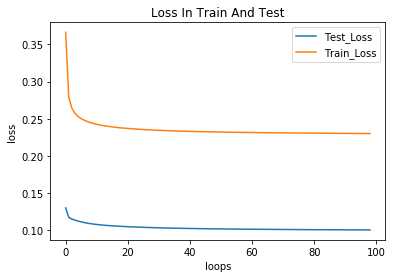
\includegraphics[width=\columnwidth]{lab4-loss}
		% Create a subtitle for the figure.
		\caption{The loss of the complete dataset u}
		% Define the label of the figure. It's good to use 'fig:title', so you know that the label belongs to a figure.
		\label{fig:tf_plot}
		\end{center}
\end{figure}
	
\begin{figure}[!hbt]
		% Center the figure.
		\begin{center}
		% Include the eps file, scale it such that it's width equals the column width. You can also put width=8cm for example...
		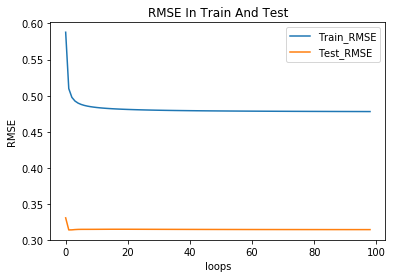
\includegraphics[width=\columnwidth]{lab4-loss-RMSE}
		% Create a subtitle for the figure.
		\caption{The RMSE of the complete dataset u}
		% Define the label of the figure. It's good to use 'fig:title', so you know that the label belongs to a figure.
		\label{fig:tf_plot}
		\end{center}
\end{figure}

\begin{figure}[!hbt]
		% Center the figure.
		\begin{center}
		% Include the eps file, scale it such that it's width equals the column width. You can also put width=8cm for example...
		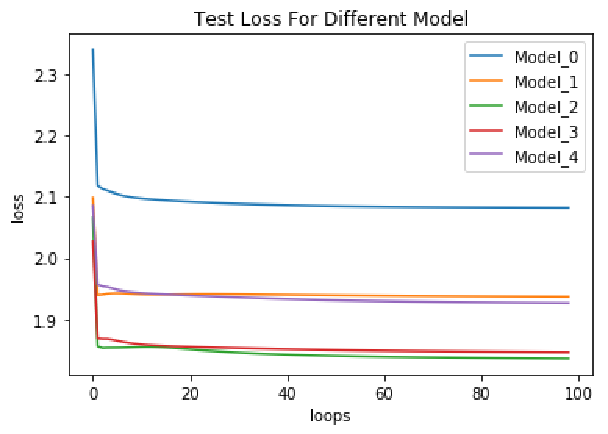
\includegraphics[width=\columnwidth]{lab4-all-loss}
		% Create a subtitle for the figure.
		\caption{The loss of all 5 divided datasets}
		% Define the label of the figure. It's good to use 'fig:title', so you know that the label belongs to a figure.
		\label{fig:tf_plot}
		\end{center}
\end{figure}

\section{Conclusion}
Through this experiment,we got a further understand of the principle of matrix decomposition as well as explored the construction of the recommended system.The use of gradient descent made us review the knowledge of gradient decent and naturally be more familiar to it.Although it cost sometime to run the experimental code,the result was of a great satisfaction to us.
% Your document ends here!
\end{document}